% !TEX root = ./Vorlesungsmitschrift AGLA 2.tex  
\lecture{Di 09.06. 10:15}{}
\file{Doppelverhältnis}
\section{Invarianten von Projektivitäten}
\begin{erinnerung*}[Das Teilverhältnis in der affinenn Geometrie]
  \( X \) ein affiner Raum über \( K \), \( p_0\neq p_1\in X \). Dann ist \( (p_0,p_1) \) eine affine Basis für die affine Gerade
  \begin{equation*}
    p_0\vee p_1\defines Y.
  \end{equation*}
  Es gibt ein eindeutig bestimmtes Koordinatensystem
  \begin{equation*}
    \varphi\maps K\to Y
  \end{equation*}
  mit \( \varphi(0)=p_0 \), \( \varphi(1)=p_1 \). Für \( p\in Y \) setzen wir
  \begin{equation*}
    \teilverhaeltnis{p_0}{p_1}{p}=\inverse{\varphi}(p).
  \end{equation*}
  \begin{beispiel*}
    \begin{figure}[H]
      \centering
      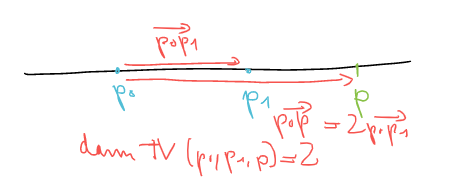
\includegraphics[width=0.5\linewidth]{teilverhaeltnis_erinnerung}
      \label{fig:teilverhaeltnis_erinnerung}
    \end{figure}
  \end{beispiel*}
  Wir können \( X \) in einen projektiven Raum \( \projectionspace{V} \) übe \( K \) einbetten (siehe letzter Abschnitt).
\end{erinnerung*}
\begin{frage*}
  Das Teilverhältnis bleibt mit Affinitäten invariant, giltdies auch für Projektivitäten, nach Einbettung in einen projektiven Raum?
\end{frage*}
\begin{beispiel*}
  Zentralprojektionen \( \pi \)
  \begin{figure}[H]
    \centering
    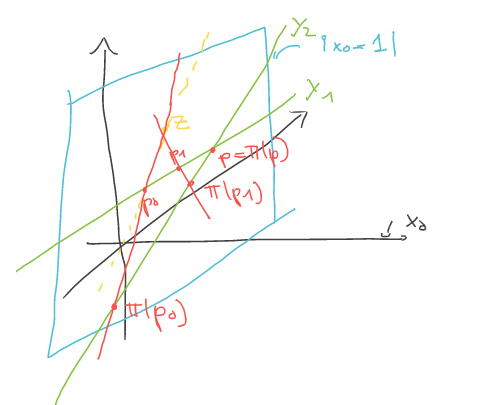
\includegraphics[width=0.5\linewidth]{zentralprojektionen_beispiel_invarianz_unter_projektivitaeten}
    \label{fig:zentralprojektionen_beispiel_invarianz_unter_projektivitaeten}
  \end{figure}
  Im Allgemeinen wird das Teilverhältnis \emph{nicht} unter Projektivitäten erhalten.
\end{beispiel*}
\begin{frage*}
  Konstruktion einer natürlichen projektiven Invarianten?
\end{frage*}
\begin{idee*}
  Wir verwenden projektive Koordinatensysteme statt affiner Koordinatensysteme.
\end{idee*}
Sei \( V \) ein \( K \)-Vektorraum und \( Z\subseteq \projectionspace{V} \) eine projektive Gerade. Dann ist \( (p_0,p_1,p_2) \)  eine projektive Basis von \( Z \) und es besteht ein eindeutig bestimmtes Koordinatensystem
\begin{equation*}
  \mathcal{K}\definedas \projectionspaceover{1}{K}\to Z
\end{equation*}
mit
\begin{align*}
  \mathcal{K}(1:0)&=p_0\\
  \mathcal{K}(0:1)&=p_1\\
  \mathcal{K}(1:1)&=p_2.
\end{align*}
Sei \( p\in Z \). Wir definieren das \emph{Doppelverhältnis} von \( p_0,p_1,p_2,p \) als
\begin{equation*}
  \doppelverhaeltnis{p_0}{p_1}{p_2}{p}\definedas \inverse{\mathcal{K}}(p)\in \projectionspaceover{1}{K}.
\end{equation*}
\begin{beispiel*}
  \( Z=\projectionspaceover{1}{K} \) mit \( p_0=(1:0) \), \( p_1=(0:1) \), \( p_2=(1:1) \). Dann ist
  \begin{equation*}
    \doppelverhaeltnis{p_0}{p_1}{p_2}{(\lambda:\mu)}=(\lambda:\mu).
  \end{equation*}
\end{beispiel*}
Das Doppelverhältnis ist invariant unter Projektivitäten:
\begin{satz}
  Seien \( V,W \) \( K \)-Vektorräume und \( f\maps \projectionspace{V}\to \projectionspace{W} \) eine Projektivität. Seien \( p_0,p_1,p_2,p\in \projectionspace{V} \) Punkte, die in einer gemeinsamen Geraden enthalten sind und \( p_0,p_1,p_2 \) paarweise verschieden. Dann gilt
  \begin{equation*}
    \doppelverhaeltnis{p_0}{p_1}{p_2}{p}=\doppelverhaeltnis{f(p_0)}{f(p_1)}{f(p_2)}{f(p)}.
  \end{equation*}
\end{satz}
\begin{proof}
  Sei \( Z\subseteq \projectionspace{V} \) die Gerade mit \( p_0,p_1,p_2,p\in Z \) und \( Z'=f(Z)\subseteq \projectionspace{W} \). Sei \( \mathcal{K}\maps \projectionspaceover{1}{K}\to K \) das Koordinatensystem mit \( \mathcal{K}(1:0)=p_0 \), \( \mathcal{K}(0:1)=p_1 \), \( \mathcal{K}(1:1)=p_2 \).
  \begin{equation*}
    \begin{tikzcd}
      &Z\arrow[name=fz,dd,"\evaluateat{f}{Z}"]\\
      \projectionspaceover{1}{K}\arrow[sloped,ur,"\mathcal{K}"]\arrow[dr,"\evaluateat{f}{Z}\circ \mathcal{K}\defines \mathcal{K}'",sloped]&\\ % ChkTeX 34
      &Z'.
    \end{tikzcd}
  \end{equation*}
  Dann ist \( \evaluateat{f}{Z}\maps Z\to Z' \) Projektivität und \( \mathcal{K}'\definedas \evaluateat{f}{Z}\circ \mathcal{K} \) eine Projektivität mit 
  \begin{align*}
    \mathcal{K}'(1:0)&=f(p_0)\\
    \mathcal{K}'(0:1)&=f(p_1)\\
    \mathcal{K}'(1:1)&=f(p_2).
  \end{align*}
  Also gilt
  \begin{align*}
    \doppelverhaeltnis{f(p_0)}{f(p_1)}{f(p_2)}{f(p)}&=\inverse{\mathcal{K'}}(f(p))\\
    &=\inverse{\mathcal{K}}(p)\\
    &=\doppelverhaeltnis{p_0}{p_1}{p_2}{p}.
  \end{align*}
\end{proof}
\file{Berechnung Doppelverhältnis}
\subsection*{Berechnung des Doppelverhältnisses aus homogenen Koordinaten}
Sei \( K \) ein Körper und seien \( p_0,p_1,p_2\in \projectionspaceover{1}{K} \) paarweise verschieden und \( p_3\in \projectionspaceover{1}{K} \). Wir nehmen an, dass \( p_0,p_1,p_2,p_3 \) in homogenen Koordinaten
\begin{equation*}
  p_i=(\lambda_i:\mu_i),\quad 0\leq i\leq 3 
\end{equation*}
gegeben sind.
\begin{ziel*}
  Berechne \( \doppelverhaeltnis{p_0}{p_1}{p_2}{p_3} \) aus \( \lambda_0,\dotsc,\lambda_3,\mu_0,\dotsc,\mu_3 \).
\end{ziel*}
\minisec{Schritt 1}
Sei \( \mathcal{K}\maps \projectionspaceover{1}{K}\to \projectionspaceover{1}{K} \) das Koordinatensystem gegeben durch
\begin{align*}
  \mathcal{K}(1:0)&=p_0\\
  \mathcal{K}(0:1)&=p_1\\
  \mathcal{K}(1:1)&=p_2.
\end{align*}
Sei \( A\maps K^2\to K^2 \) ein Isomorphismus mit Matrix \( A\in \invertiblematrices{2}{K} \) und \( \projectionspace{A}=\mathcal{K} \). Wir bestimmen explizit eine solche Matrix \( A \). Aus 
\begin{equation*}
  A\begin{pmatrix} 1 \\ 0 \end{pmatrix}\in \fieldwithoutzero{K}\cdot \begin{pmatrix} \lambda_0 \\ \mu_0 \end{pmatrix}
\end{equation*}
und
\begin{equation*}
  A\begin{pmatrix} 0 \\ 1 \end{pmatrix}\in \fieldwithoutzero{K}\begin{pmatrix} \lambda_1 \\ \mu_1 \end{pmatrix}
\end{equation*}
folgt, dass es \( \rho,\rho'\in \fieldwithoutzero{K} \) gibt mit
\begin{equation*}
  A=\begin{pmatrix} \rho \lambda_0 & \rho' \lambda_1 \\ \rho \mu_0 & \rho' \mu_1 \end{pmatrix}.
\end{equation*}
Aus \( \mathcal{K}(1:1)=p_2 \) folgt
\begin{equation*}
  \left.\begin{aligned}
    \rho\lambda_0 +\rho'\lambda_1&=\rho''\lambda_2\\
    \rho\mu_0+\rho'\mu_1&=\rho'' \mu_2
  \end{aligned}\right\}\label{eq:bestimmende_gleichung_matrix_projektive_koordinaten}\tag{*}
\end{equation*}
für ein \( \rho''\in \fieldwithoutzero{K} \). Das System \eqref{eq:bestimmende_gleichung_matrix_projektive_koordinaten} kann \zb gelöst werden durch
\begin{align*}
  \rho''&=\det \begin{pmatrix} \lambda_0 & \lambda_1 \\ \mu_0 & \mu_1 \end{pmatrix}\\
    \rho&=\det \begin{pmatrix} \lambda_2 & \lambda_1 \\ \mu_2 & \mu_1 \end{pmatrix}\\
    \rho'&=\det \begin{pmatrix} \lambda_0 & \lambda_1 \\ \mu_0 & \mu_1 \end{pmatrix}.
\end{align*}
Dann ist
\begin{equation*}
  A=\begin{pmatrix} \lambda_0 \det \begin{pmatrix} \lambda_2 & \lambda_1 \\ \mu_2 & \mu_1 \end{pmatrix} & \lambda_1 \det \begin{pmatrix} \lambda_0 & \lambda_2 \\ \mu_0 & \mu_2 \end{pmatrix} \\ \mu_0 \det \begin{pmatrix} \lambda_2 & \lambda_1 \\ \mu_2 & \mu_1 \end{pmatrix} & \mu_1 \det \begin{pmatrix} \lambda_0 & \lambda_2 \\ \mu_0 & \mu_2 \end{pmatrix} \end{pmatrix}
\end{equation*}
und \( \inverse{K}\maps \projectionspaceover{1}{K}\to\projectionspaceover{1}{K} \) gegebene durch \( \inverse{K}=\projectionmap{\inverse{A}} \) mit
\begin{equation*}
  \inverse{A}=\frac{1}{\det A}\begin{pmatrix}
    \mu_1 \det \begin{pmatrix} \lambda_0 & \lambda_2 \\ \mu_0 & \mu_2 \end{pmatrix} & -\lambda_1 \det \begin{pmatrix} \lambda_0 & \lambda_2 \\ \mu_0 & \mu_2 \end{pmatrix} \\
    -\mu_0 \det \begin{pmatrix} \lambda_2 & \lambda_1 \\ \mu_2 & \mu_1 \end{pmatrix} & \lambda_0 \det \begin{pmatrix} \lambda_2 & \lambda_1 \\ \mu_2 & \mu_1 \end{pmatrix}
  \end{pmatrix}.
\end{equation*}
Wir berechnen
\begin{align*}
  \inverse{\mathcal{K}}(\lambda_3:\mu_3)&=K\cdot\cdot\inverse{A}\begin{pmatrix} \lambda_3 \\ \mu_3 \end{pmatrix}\\
  &=K\cdot \begin{pmatrix}\det \begin{pmatrix} \lambda_0 & \lambda_2 \\ \mu_0 & \mu_2 \end{pmatrix}\cdot \det \begin{pmatrix} \lambda_3 & \lambda_1 \\ \mu_3 & \mu_1 \end{pmatrix} \\ \det \begin{pmatrix} \lambda_2 & \lambda_1 \\ \mu_2 & \mu_1 \end{pmatrix}\cdot\det \begin{pmatrix} \lambda_3 & \lambda_0 \\ \mu_3 & \mu_0 \end{pmatrix} \end{pmatrix}.
\end{align*}
Wir formulieren das Resultat im folgenden Lemma:
\begin{lemma}\label{doppelverhaeltnis_berechnung}
  Seien \( p_0,p_1,p_2,p_3\in \projectionspaceover{1}{K} \) mit \( p_0,p_1,p_2 \) paarweise verschieden und
  \begin{equation*}
    p_i=(\lambda_i:\mu_i),\quad 0\leq i\leq 3-
  \end{equation*}
  Dann gilt
  \begin{align*}
    \doppelverhaeltnis{p_0}{p_1}{p_2}{p_3}=\parens*{\det\begin{pmatrix} \lambda_2 & \lambda_0 \\ \mu_2 & \mu_0 \end{pmatrix}\det \begin{pmatrix} \lambda_3 & \lambda_1 \\ \mu_3 & \mu_1 \end{pmatrix}:\det \begin{pmatrix} \lambda_2 & \lambda_1 \\ \mu_2 & \mu_1 \end{pmatrix}\det \begin{pmatrix} \lambda_3 & \lambda_0 \\ \mu_3 & \mu_0 \end{pmatrix}}.
  \end{align*}
\end{lemma}
\begin{beispiel*}
  Seien \( p_0,p_1,p_2\in \projectionspaceover{1}{K} \) paarweise verschieden. Nach \thref{doppelverhaeltnis_berechnung} ist 
  \begin{equation*}
    \doppelverhaeltnis{p_0}{p_1}{p_2}{p}=\begin{pmatrix} 0 & 1 \end{pmatrix}
  \end{equation*}
  genau dann, wenn
  \begin{equation*}
    \det \begin{pmatrix} \lambda_3 & \lambda_1 \\ \mu_3 & \mu_1 \end{pmatrix}=0
  \end{equation*}
  \dh \( (\lambda_3:\mu_3)=(\lambda_1:\mu_1) \). Wir erhalten also die Aussage zurück
  \begin{equation*}
    \doppelverhaeltnis{p_0}{p_1}{p_2}{p}=(0:1)
  \end{equation*}
  genau dann, wenn \( p_1=p \).
\end{beispiel*}
\begin{bemerkung*}
  Aus \thref{doppelverhaeltnis_berechnung} können wir  weitere Symmetrieeigenschaften des Doppelverhältnisses ableiten. Seien dazu \( p_0,p_1,p_2,p \) paarweise verschieden. Dann ist \zb
  \begin{equation*}
    \doppelverhaeltnis{p_0}{p_1}{p_2}{p_3}=\doppelverhaeltnis{p_1}{p_0}{p_3}{p_2},
  \end{equation*}
  denn
  \begin{equation*}
    \doppelverhaeltnis{p_0}{p_1}{p_2}{p_3}=(s:t)
  \end{equation*}
  ist äquivalent zu 
  \begin{equation*}
    \doppelverhaeltnis{p_1}{p_0}{p_2}{p_3}=(t:s).
  \end{equation*}
\end{bemerkung*}
\begin{frage*}
  Sei \( n\geq 1 \), \( p_0, p_1,p_2,p_3\in \projectionspaceover{n}{K} \) in einer Geraden enthalten mit \( p_0,p_1,p_2 \) paarweise verschieden und 
  \begin{equation*}
    p_i=(x_0^{(i)}:x_1^{(i)}:\dotsc:x_n^{(i)}) \quad 0\leq i\leq 3
  \end{equation*}
  in homogenen Koordinaten. Wie können wir aus den homogenen Koordinaten \( \doppelverhaeltnis{p_0}{p_1}{p_2}{p_3}  \) berechnen?
\end{frage*}
\begin{idee*}
  Sei \( Z\subseteq \projectionspaceover{n}{K} \) die projektive Gerade, die \( p_0,p_1,p_2,p_3 \) enthält. Verwende eine Zentralprojektion
  \begin{equation*}
    f\maps Z\to \explain{\text{einer der projektiven Unterräume \( \projectionspace{\set{(x_0,\dotsc,x_n)\in K^{n+1}|x_k=0 \text{ für } k\not\in \set{i,j}}} \) für \( i\neq j \)}}{\projectionspaceover{1}{K}}\subseteq \projectionspaceover{n}{K}
  \end{equation*}
  um das Problem auf den eindimensionalen Fall zurückzuführen durch
  \begin{equation*}
    \doppelverhaeltnis{p_0}{p_1}{p_2}{p_3}=\doppelverhaeltnis{f(p_0)}{f(p_1)}{f(p_2)}{f(p_3)}.
  \end{equation*}
  Sei \( Z=\projectionspace{W} \) mit \( W\subseteq K^{n+1} \) \( 2 \)-dimensionaler \( K \)-Untervektorraum. Sei für \( i\neq j \)
  \begin{equation*}
    V_{ij}=\set{(x_0,\dotsc,x_n)\in K^{n+1}|x_k=0 \text{für} k\not\in \set{i,j}}
  \end{equation*}
  und
  \begin{equation*}
    \hat{V}_{ij}=\set{(x_0,\dotsc,x_n)\in K^{n+1}|x_i=x_j=0}.
  \end{equation*}
  Dann ist \( K^{n+1}=V_{ij}\oplus \hat{V}_{ij} \) und die Projektion
  \begin{equation*}
    P\maps \equalto{V_{ij}\oplus \hat{V}_{ij}}{K^{n+1}}\to V_{ij}
  \end{equation*}
  induziert eine Zentralprojektion
  \begin{equation*}
    f\maps Z\to \projectionspace{V_{ij}}
  \end{equation*}
  genau dann, wenn
  \begin{equation*}
    K^{n+1}=W\oplus \hat{V}_{ij}.
  \end{equation*}
  Aus Dimensionsgründen ist dies äquivalent zu
  \begin{equation*}
    K^{n+1}=W+\hat{V}_{ij}.
  \end{equation*}
\end{idee*}
\begin{lemma}
  Seien \( p_0,p_1,p_2,p_3\in \projectionspaceover{n}{K} \) in einer Gerade enthalten und \( p_0,p_1,p_2 \) paarweise verschieden. Sei
  \begin{equation*}
    p_k=(x_0^{(k)}:\dotsc:x_n^{(k)})\quad 0\leq k\leq 3
  \end{equation*}
  in homogenen Koordinaten.

  Seien \( 1\leq i,j\leq n \), \( i\neq j \) gegeben mit
  \begin{equation*}
    \det \begin{pmatrix} x_i^{(0)} & x_i^{(1)} \\ x_j^{(0)} & x_j^{(1)} \end{pmatrix}\neq 0.
  \end{equation*}
  Dann gilt
  \begin{equation*}
    \doppelverhaeltnis{p_0}{p_1}{p_2}{p_3}=\parens*{\det \begin{pmatrix} x_i^{(2)} & x_i^{(0)} \\ x_j^{(2)} & x_j^{(0)} \end{pmatrix}\det \begin{pmatrix} x_i^{(3)} & x_i^{(1)} \\ x_j^{(3)} & x_j^{(1)} \end{pmatrix}:\det \begin{pmatrix} x_i^{(2)} & x_i^{(1)} \\ x_j^{(2)} & x_j^{(1)} \end{pmatrix}\det \begin{pmatrix} x_i^{(3)} & x_i^{(0)} \\ x_j^{(3)} & x_j^{(0)} \end{pmatrix}}.
  \end{equation*}
\end{lemma}
\lecture{Fr 12.06. 10:15}{}
\subsection*{Zusammenhang Doppelverhältnis \( \leftrightarrow \) Teilverhältnis}
Seien \( p_0,p_1,p_2,p_3\in \projectionspaceover{1}{K} \) paarweise
verschieden und \( p_i=(1:\mu_i) \) für \( 0\leq i\leq 3 \) (wir schließen also hier den Punkt \( (0:1) \) aus). Dann gilt nach \thref{doppelverhaeltnis_berechnung}
\begin{align*}
  \doppelverhaeltnis{p_0}{p_1}{p_2}{p_3}&=\parens*{\braceannotate{\neq 0}{(\mu_0-\mu_2)}(\mu_1-\mu_3):(\mu_1-\mu_2)\braceannotate{\neq 0}{(\mu_0-\mu3)}}\\
  &=\parens*{\frac{\mu_1-\mu_3}{\mu_0-\mu_3}:\frac{\mu_1-\mu_2}{\mu_0-\mu_2}}\\
  &=(\teilverhaeltnis{\mu_3}{\mu_0}{\mu_1}:\teilverhaeltnis{\mu_2}{\mu_0}{\mu_1}).
\end{align*}
Also können wir in diesem Fall das Doppelverhältnis als \enquote{Verhältnis von Teilverhältnissen} verstehen.
\begin{bemerkungen*}
  Ist \( p_0=(0:1) \) und \( p_i=(1:\mu_i) \) für \( 1\leq i\leq 3 \) paarweise verschieden, so gilt nach \thref{doppelverhaeltnis_berechnung}
  \begin{align*}
    \doppelverhaeltnis{p_0}{p_1}{p_2}{p_3}&=(\mu_1-\mu_3:\mu_1-\mu_2)\\
    &=\parens*{\frac{\mu_3-\mu_1}{\mu_2-\mu_1}:1}\\
    &=(\teilverhaeltnis{\mu_1}{\mu_2}{\mu_3}:1).
  \end{align*}
\end{bemerkungen*}